\documentclass[tikz, border=6pt]{standalone}
\usepackage[T1]{fontenc}
\usepackage{lmodern}
\usepackage{amsmath,amssymb,bm}
\usepackage[scaled=0.95]{helvet}
\usetikzlibrary{arrows.meta}
\definecolor{Blue}{HTML}{3A76D8}
\definecolor{Green}{HTML}{3BA55C}
\definecolor{Yellow}{HTML}{EAB531}
\definecolor{Red}{HTML}{DF4B4B}
\definecolor{Purple}{HTML}{8459D1}
\definecolor{Ink}{HTML}{1F2937}
\begin{document}
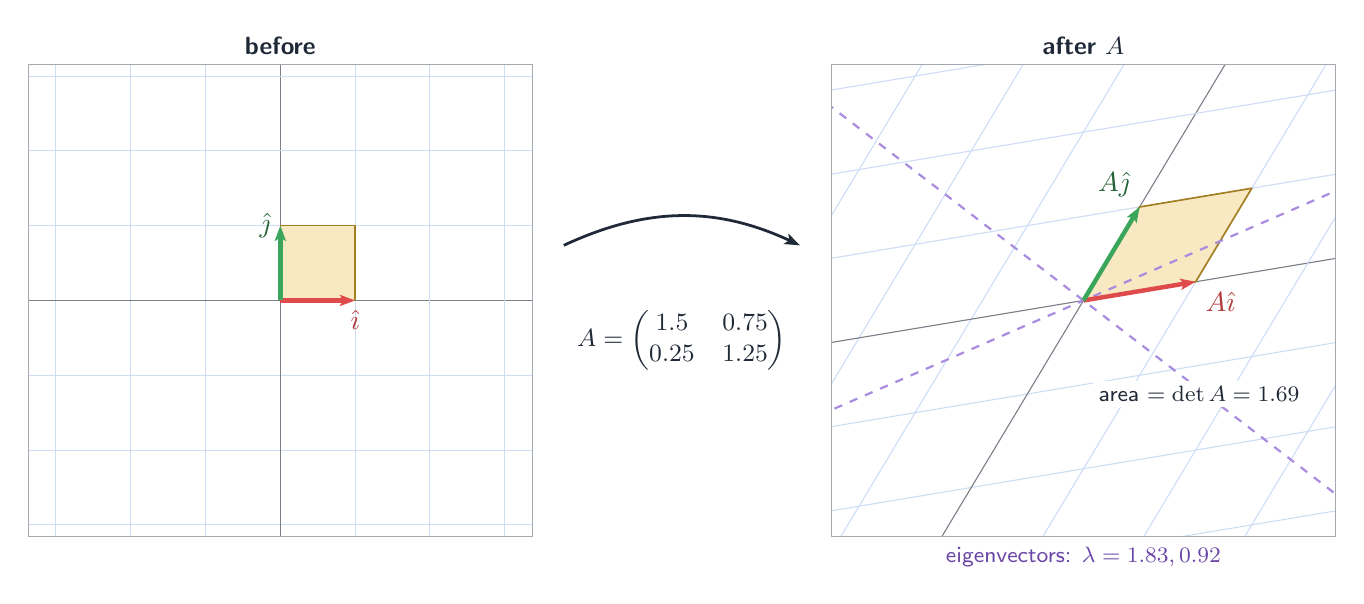
\begin{tikzpicture}[color=Ink, execute at begin picture={\sffamily}, line width=0.6pt, >={Stealth[length=5.5pt, width=4pt, inset=1.2pt]}, line join=round]
  \begin{scope}
    \clip (-3.2,-3) rectangle (3.2,3);
    \draw[color=Blue!25, line width=0.4pt] (-7.6,-7.6) -- (-7.6,7.6);
    \draw[color=Blue!25, line width=0.4pt] (-7.6,-7.6) -- (7.6,-7.6);
    \draw[color=Blue!25, line width=0.4pt] (-6.65,-7.6) -- (-6.65,7.6);
    \draw[color=Blue!25, line width=0.4pt] (-7.6,-6.65) -- (7.6,-6.65);
    \draw[color=Blue!25, line width=0.4pt] (-5.7,-7.6) -- (-5.7,7.6);
    \draw[color=Blue!25, line width=0.4pt] (-7.6,-5.7) -- (7.6,-5.7);
    \draw[color=Blue!25, line width=0.4pt] (-4.75,-7.6) -- (-4.75,7.6);
    \draw[color=Blue!25, line width=0.4pt] (-7.6,-4.75) -- (7.6,-4.75);
    \draw[color=Blue!25, line width=0.4pt] (-3.8,-7.6) -- (-3.8,7.6);
    \draw[color=Blue!25, line width=0.4pt] (-7.6,-3.8) -- (7.6,-3.8);
    \draw[color=Blue!25, line width=0.4pt] (-2.85,-7.6) -- (-2.85,7.6);
    \draw[color=Blue!25, line width=0.4pt] (-7.6,-2.85) -- (7.6,-2.85);
    \draw[color=Blue!25, line width=0.4pt] (-1.9,-7.6) -- (-1.9,7.6);
    \draw[color=Blue!25, line width=0.4pt] (-7.6,-1.9) -- (7.6,-1.9);
    \draw[color=Blue!25, line width=0.4pt] (-0.95,-7.6) -- (-0.95,7.6);
    \draw[color=Blue!25, line width=0.4pt] (-7.6,-0.95) -- (7.6,-0.95);
    \draw[color=Ink!60, line width=0.4pt] (0,-7.6) -- (0,7.6);
    \draw[color=Ink!60, line width=0.4pt] (-7.6,0) -- (7.6,0);
    \draw[color=Blue!25, line width=0.4pt] (0.95,-7.6) -- (0.95,7.6);
    \draw[color=Blue!25, line width=0.4pt] (-7.6,0.95) -- (7.6,0.95);
    \draw[color=Blue!25, line width=0.4pt] (1.9,-7.6) -- (1.9,7.6);
    \draw[color=Blue!25, line width=0.4pt] (-7.6,1.9) -- (7.6,1.9);
    \draw[color=Blue!25, line width=0.4pt] (2.85,-7.6) -- (2.85,7.6);
    \draw[color=Blue!25, line width=0.4pt] (-7.6,2.85) -- (7.6,2.85);
    \draw[color=Blue!25, line width=0.4pt] (3.8,-7.6) -- (3.8,7.6);
    \draw[color=Blue!25, line width=0.4pt] (-7.6,3.8) -- (7.6,3.8);
    \draw[color=Blue!25, line width=0.4pt] (4.75,-7.6) -- (4.75,7.6);
    \draw[color=Blue!25, line width=0.4pt] (-7.6,4.75) -- (7.6,4.75);
    \draw[color=Blue!25, line width=0.4pt] (5.7,-7.6) -- (5.7,7.6);
    \draw[color=Blue!25, line width=0.4pt] (-7.6,5.7) -- (7.6,5.7);
    \draw[color=Blue!25, line width=0.4pt] (6.65,-7.6) -- (6.65,7.6);
    \draw[color=Blue!25, line width=0.4pt] (-7.6,6.65) -- (7.6,6.65);
    \draw[color=Blue!25, line width=0.4pt] (7.6,-7.6) -- (7.6,7.6);
    \draw[color=Blue!25, line width=0.4pt] (-7.6,7.6) -- (7.6,7.6);
    \draw[fill=Yellow!35, draw=Yellow!70!black, line width=0.6pt, fill opacity=0.85] (0,0) -- (0.95,0)
        -- (0.95,0.95) -- (0,0.95) -- cycle;
    \draw[->, color=Red, line width=1.6pt] (0,0) -- (0.95,0);
    \draw[->, color=Green, line width=1.6pt] (0,0) -- (0,0.95);
  \end{scope}
  \draw[draw=Ink!40, line width=0.5pt] (-3.2,-3) rectangle (3.2,3);
  \node[anchor=south, font=\small\bfseries] at (0,3) {before};
  \begin{scope}
    \clip (7,-3) rectangle (13.4,3);
    \draw[color=Blue!25, line width=0.4pt] (-6.9,-11.4) -- (4.5,7.6);
    \draw[color=Blue!25, line width=0.4pt] (-6.9,-11.4) -- (15.9,-7.6);
    \draw[color=Blue!25, line width=0.4pt] (-5.475,-11.1625) -- (5.925,7.8375);
    \draw[color=Blue!25, line width=0.4pt] (-6.1875,-10.2125) -- (16.6125,-6.4125);
    \draw[color=Blue!25, line width=0.4pt] (-4.05,-10.925) -- (7.35,8.075);
    \draw[color=Blue!25, line width=0.4pt] (-5.475,-9.025) -- (17.325,-5.225);
    \draw[color=Blue!25, line width=0.4pt] (-2.625,-10.6875) -- (8.775,8.3125);
    \draw[color=Blue!25, line width=0.4pt] (-4.7625,-7.8375) -- (18.0375,-4.0375);
    \draw[color=Blue!25, line width=0.4pt] (-1.2,-10.45) -- (10.2,8.55);
    \draw[color=Blue!25, line width=0.4pt] (-4.05,-6.65) -- (18.75,-2.85);
    \draw[color=Blue!25, line width=0.4pt] (0.225,-10.2125) -- (11.625,8.7875);
    \draw[color=Blue!25, line width=0.4pt] (-3.3375,-5.4625) -- (19.4625,-1.6625);
    \draw[color=Blue!25, line width=0.4pt] (1.65,-9.975) -- (13.05,9.025);
    \draw[color=Blue!25, line width=0.4pt] (-2.625,-4.275) -- (20.175,-0.475);
    \draw[color=Blue!25, line width=0.4pt] (3.075,-9.7375) -- (14.475,9.2625);
    \draw[color=Blue!25, line width=0.4pt] (-1.9125,-3.0875) -- (20.8875,0.7125);
    \draw[color=Ink!60, line width=0.4pt] (4.5,-9.5) -- (15.9,9.5);
    \draw[color=Ink!60, line width=0.4pt] (-1.2,-1.9) -- (21.6,1.9);
    \draw[color=Blue!25, line width=0.4pt] (5.925,-9.2625) -- (17.325,9.7375);
    \draw[color=Blue!25, line width=0.4pt] (-0.4875,-0.7125) -- (22.3125,3.0875);
    \draw[color=Blue!25, line width=0.4pt] (7.35,-9.025) -- (18.75,9.975);
    \draw[color=Blue!25, line width=0.4pt] (0.225,0.475) -- (23.025,4.275);
    \draw[color=Blue!25, line width=0.4pt] (8.775,-8.7875) -- (20.175,10.2125);
    \draw[color=Blue!25, line width=0.4pt] (0.9375,1.6625) -- (23.7375,5.4625);
    \draw[color=Blue!25, line width=0.4pt] (10.2,-8.55) -- (21.6,10.45);
    \draw[color=Blue!25, line width=0.4pt] (1.65,2.85) -- (24.45,6.65);
    \draw[color=Blue!25, line width=0.4pt] (11.625,-8.3125) -- (23.025,10.6875);
    \draw[color=Blue!25, line width=0.4pt] (2.3625,4.0375) -- (25.1625,7.8375);
    \draw[color=Blue!25, line width=0.4pt] (13.05,-8.075) -- (24.45,10.925);
    \draw[color=Blue!25, line width=0.4pt] (3.075,5.225) -- (25.875,9.025);
    \draw[color=Blue!25, line width=0.4pt] (14.475,-7.8375) -- (25.875,11.1625);
    \draw[color=Blue!25, line width=0.4pt] (3.7875,6.4125) -- (26.5875,10.2125);
    \draw[color=Blue!25, line width=0.4pt] (15.9,-7.6) -- (27.3,11.4);
    \draw[color=Blue!25, line width=0.4pt] (4.5,7.6) -- (27.3,11.4);
    \draw[fill=Yellow!35, draw=Yellow!70!black, line width=0.6pt, fill opacity=0.85] (10.2,0) --
        (11.625,0.2375) -- (12.3375,1.425) -- (10.9125,1.1875) -- cycle;
    \draw[color=Purple!70, dashed, line width=0.8pt] (0.6547,-4.1451) -- (19.7453,4.1451);
    \draw[color=Purple!70, dashed, line width=0.8pt] (14.3793,-3.208) -- (6.0207,3.208);
    \draw[->, color=Red, line width=1.6pt] (10.2,0) -- (11.625,0.2375);
    \draw[->, color=Green, line width=1.6pt] (10.2,0) -- (10.9125,1.1875);
  \end{scope}
  \draw[draw=Ink!40, line width=0.5pt] (7,-3) rectangle (13.4,3);
  \node[anchor=south, font=\small\bfseries] at (10.2,3) {after $A$};
  \node[anchor=north, text=Red!80!black] at (0.95,0) {$\hat\imath$};
  \node[anchor=east, text=Green!60!black] at (0,0.95) {$\hat\jmath$};
  \node[anchor=north west, text=Red!80!black] at (11.625,0.2375) {$A\hat\imath$};
  \node[anchor=south east, text=Green!60!black] at (10.9125,1.1875) {$A\hat\jmath$};
  \node[font=\footnotesize, fill=white, inner sep=2pt] at (11.6687,-1.1875) {area $= \det A = 1.69$};
  \draw[->, line width=1pt] (3.6,0.7) to[bend left=25] (6.6,0.7);
  \node[font=\small] at (5.1,-0.5) {$A = \begin{pmatrix} 1.5 & 0.75 \\ 0.25 & 1.25 \end{pmatrix}$};
  \node[anchor=north, font=\footnotesize, text=Purple!80!black] at (10.2,-3) {eigenvectors: $\lambda = 1.83, 0.92$};
\end{tikzpicture}
\end{document}
